\documentclass{article}
\usepackage{lmodern}
\usepackage[most]{tcolorbox}
\usepackage{lipsum}
\usepackage[top=.5in, left=.5in, right=.5in, bottom=.5in]{geometry}

\tcbset{
    mybox/.style={
        enhanced,
        attach boxed title to top left={yshift*=-\tcboxedtitleheight},
        coltitle=black,
        colframe=#1,
        colback=#1!10,
        boxed title style={
            size=small,
            colback=#1!30},
        }
}

\newcommand{\WS}[4][Problem]{%
\begin{tcbitemize}[%
    raster force size=false,
    raster equal height=rows,
    raster row skip=0pt,
    raster column skip=0pt,
    raster row 1/.style={
        mybox=orange,
        raster multicolumn=2,
        notitle},
    raster row 2 column 1/.style={%
        mybox= red,
        add to width= .05\textwidth,
        title=Question},
    raster row 2 column 2/.style={%
        mybox= blue,
        add to width= -.05\textwidth,
        title=Hint},
    raster row 3 column 1/.style={%
        mybox= green,
        raster multicolumn=2, 
        height fill,
        title=Answer},  
    ]
\tcbitem \textbf{#1}\hfill\thepage
\tcbitem #2 
\tcbitem #3
\tcbitem #4
\end{tcbitemize}}

\pagestyle{empty}
\begin{document}
\WS{Suppose you have a right triangle as presented below.  Let $a=2$ cm, and $b=3$ cm.  How long would $c$ be? 
        {\par\centering
        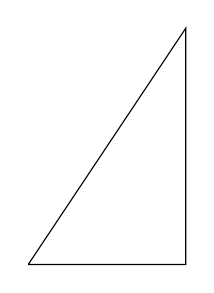
\begin{tikzpicture}
            \draw[rounded corners=0pt] (0,0) -- (2,0) -- (2,3) -- (0,0);
        \end{tikzpicture}
        \par}
        Remember to leave your answers as a square root, and to show all work and leave units.}%
{  \begin{itemize}
      \item Think about the pythagorean formula.
      \item It involves squares.
      \item And adding.
  \end{itemize}}{This is my answer

  \lipsum[1]}

\end{document}